% ------------------------------------------------------------------------
% ------------------------------------------------------------------------
% abnTeX2: Modelo de Trabalho Academico (tese de doutorado, dissertacao de
% mestrado e trabalhos monograficos em geral) em conformidade com 
% ABNT NBR 14724:2011: Informacao e documentacao - Trabalhos academicos -
% Apresentacao
% ------------------------------------------------------------------------
% ------------------------------------------------------------------------

\documentclass[
	% -- opções da classe memoir --
	12pt,				% tamanho da fonte
	openright,			% capítulos começam em pág ímpar (insere página vazia caso preciso)
	%twoside,			% para impressão em verso e anverso. Oposto a oneside
	oneside,
	a4paper,			% tamanho do papel. 
	% -- opções da classe abntex2 --
	%chapter=TITLE,		% títulos de capítulos convertidos em letras maiúsculas
	%section=TITLE,		% títulos de seções convertidos em letras maiúsculas
	%subsection=TITLE,	% títulos de subseções convertidos em letras maiúsculas
	%subsubsection=TITLE,% títulos de subsubseções convertidos em letras maiúsculas
	% -- opções do pacote babel --
	english,			% idioma adicional para hifenização
	french,				% idioma adicional para hifenização
	spanish,			% idioma adicional para hifenização
	brazil				% o último idioma é o principal do documento
	]{abntex2}

% ---
% Pacotes básicos 
% ---
\usepackage{lmodern}			% Usa a fonte Latin Modern			
\usepackage[T1]{fontenc}		% Selecao de codigos de fonte.
\usepackage[utf8]{inputenc}		% Codificacao do documento (conversão automática dos acentos)
\usepackage{lastpage}			% Usado pela Ficha catalográfica
\usepackage{indentfirst}		% Indenta o primeiro parágrafo de cada seção.
\usepackage{color}				% Controle das cores
\usepackage{graphicx}			% Inclusão de gráficos
\usepackage{microtype} 			% para melhorias de justificação
\usepackage[font={small,it}]{caption}

% ---
		
% ---
% Pacotes adicionais, usados apenas no âmbito do Modelo Canônico do abnteX2
% ---
\usepackage{lipsum}				% para geração de dummy text
% ---

% ---
% Pacotes de citações
% ---
\usepackage[brazilian,hyperpageref]{backref}	 % Paginas com as citações na bibl
\usepackage[alf]{abntex2cite}	% Citações padrão ABNT

% define o caminho das imagens
\graphicspath{{Imagens/}}

% --- 
% CONFIGURAÇÕES DE PACOTES
% --- 

% ---
% Configurações do pacote backref
% Usado sem a opção hyperpageref de backref
\renewcommand{\backrefpagesname}{Citado na(s) página(s):~}
% Texto padrão antes do número das páginas
\renewcommand{\backref}{}
% Define os textos da citação
\renewcommand*{\backrefalt}[4]{
	\ifcase #1 %
		Nenhuma citação no texto.%
	\or
		Citado na página #2.%
	\else
		Citado #1 vezes nas páginas #2.%
	\fi}%
% ---

\newcommand{\monoTitulo}{Utilização de Clusterização Fuzzy e Redes Neurais Artificiais para Prevenção de Intrusao} 
\newcommand{\monoIDS}{\textit{Intrusion Detection System} } 
\newcommand{\monoIPS}{\textit{Intrusion Prevention System} }
\newcommand{\monoFireWall}{\textit{firewall}}


% ---
% Informações de dados para CAPA e FOLHA DE ROSTO
% ---
\titulo{Utilização de Clusterização Fuzzy e Redes Neurais Artificiais para Prevenção de Intrusao}
\autor{Rodrigo Mendonça da Paixão \\ Lucas Teles Agostinho}
\local{São Paulo -- Brasil}
\data{2015}
\orientador{Eduardo Heredia}
%\coorientador{Nome Completo}
\instituicao{%
  Centro Universitário Senac
  \par
  Bacharelado em Ciência da Computação
}
\tipotrabalho{Monografia (Graduação)}
% O preambulo deve conter o tipo do trabalho, o objetivo, 
% o nome da instituição e a área de concentração 
\preambulo{Pré-monografia apresentada na disciplina Trabalho de Conclusão de Curso I, como parte dos requisitos para obtenção do título de Bacharel em Ciência da Computação.}
% ---

% ---
% Configurações de aparência do PDF final

% alterando o aspecto da cor azul
\definecolor{blue}{RGB}{41,5,195}

% informações do PDF
\makeatletter
\hypersetup{
     	%pagebackref=true,
		pdftitle={\@title}, 
		pdfauthor={\@author},
    	pdfsubject={\imprimirpreambulo},
	    pdfcreator={LaTeX with abnTeX2},
		pdfkeywords={abnt}{latex}{abntex}{abntex2}{trabalho acadêmico}, 
		colorlinks=true,       		% false: boxed links; true: colored links
    	linkcolor=blue,          	% color of internal links
    	citecolor=blue,        		% color of links to bibliography
    	filecolor=magenta,      		% color of file links
		urlcolor=blue,
		bookmarksdepth=4
}
\makeatother
% --- 

% --- 
% Espaçamentos entre linhas e parágrafos 
% --- 

% O tamanho do parágrafo é dado por:
\setlength{\parindent}{1.3cm}

% Controle do espaçamento entre um parágrafo e outro:
\setlength{\parskip}{0.2cm}  % tente também \onelineskip

% ---
% compila o indice
% ---
\makeindex
% ---

% ----
% Início do documento
% ----
\begin{document}

% Retira espaço extra obsoleto entre as frases.
\frenchspacing 

% ----------------------------------------------------------
% ELEMENTOS PRÉ-TEXTUAIS
% ----------------------------------------------------------
% \pretextual

% ---
% Capa
% ---
\imprimircapa
% ---

% ---
% Folha de rosto
% (o * indica que haverá a ficha bibliográfica)
% ---
\imprimirfolhaderosto%*
% ---

% ---
% RESUMOS
% ---

% resumo em português
\setlength{\absparsep}{18pt} % ajusta o espaçamento dos parágrafos do resumo
%\begin{resumo}
   
 %\textbf{Palavras-chaves}: IDS,Rede,Internet
%\end{resumo}

% ---
% inserir lista de ilustrações (figuras)
% ---
%\pdfbookmark[0]{\listfigurename}{lof}
%\listoffigures*
%\cleardoublepage
% ---

% ---
% inserir lista de tabelas
% ---
%\pdfbookmark[0]{\listtablename}{lot}
%\listoftables*
%\cleardoublepage
% ---

% ---
% inserir lista de abreviaturas e siglas
% ---
\begin{siglas}
  \item[IDS] Intrusion Detection System
  \item[IPS] Intrusion Prevention System
  \item[NIDS] Network Intrusion Detection System
  \item[RNA] Rede Neural Artificial
  \item[SVM] Suport Vector Machine
  \item[AI] Artificial Intelligence
  \item[ML] Machine Learning
  \item[PNN] Rede Neural Probabilística
  \item[MLP] Multi-layered Perceptron  
\end{siglas}
% ---

% ---
% inserir o sumario
% ---
\pdfbookmark[0]{\contentsname}{toc}
\tableofcontents*
\cleardoublepage
% ---

% ----------------------------------------------------------
% ELEMENTOS TEXTUAIS 
% ----------------------------------------------------------
\textual

% ----------------------------------------------------------
% Capitulo 1
% ----------------------------------------------------------

\chapter[Introdução]{Introdução}
%\addcontentsline{toc}{chapter}{Introdução}
% ----------------------------------------------------------
Este trabalho aborda Sistemas de detecção de intrusão (\monoIDS ou IDS) e Sistemas de prevenção de intrusão (\monoIPS ou IPS), explora a utilização de técnicas de inteligencia artificial e classificação com foco em Redes Neurais Artificiais (RNA). Com o titulo "\monoTitulo"  foi desenvolvido no Centro universitário Senac em comprimento dos requisitos para graduação em ciência da computação. Supervisionado pelo Prof. Dr. Eduardo Heredia.

Desejamos abordar o funcionamento dos IDS atuais, suas limitações, como se comportam e a importância da utilização de técnicas de IA em seu escopo.
	
\section{Motivação}

A definição básica para um incidente de intrusão pode ser definida como ações que comprometam os princípios da segurança da informação, Esses princípios são definidos como Confidencialidade, Integridade e Disponibilidade de recursos computacionais e de rede \cite{whitman2011principles}. 

Detecção de intrusão é o processo de se identificar e responder a essas atividades de intrusão. Como o aumento da utilização da internet para  as tarefas do dia a dia tem se tornado mais comum, tendo crescimento tanto na quantidade de usuários quanto nas tarefas possíveis de serem realizadas a utilizando, com isso também temos um aumento no risco de incidentes de quebra de segurança. Segundo o CERT \cite{CERT} tivemos um crescimento de 197\% de incidentes reportados no ano de 2014 relativo a 2013. 

Muitos informação sigilosa pode ser trafegada na rede, pessoas e empresas podem fazer transações bancarias, \textit{backup} de dados pessoais, informação de mercado, dentre outras. Em muitos casos o \monoFireWall não é suficiente para garantir a segurança. Também existem casos de usuários de dentro da rede que abusam de seus privilégios para obter informações indevidamente ou de ataques que simplesmente não são reconhecidos pelo sistema de detecção que esta monitorando.

Incluímos alguns gráficos para demonstrar a difusão, motivações, técnicas e alvos por trás dos ataques registrados no ano de 2014:



\begin{figure}
	\begin{minipage}{.5\textwidth}
	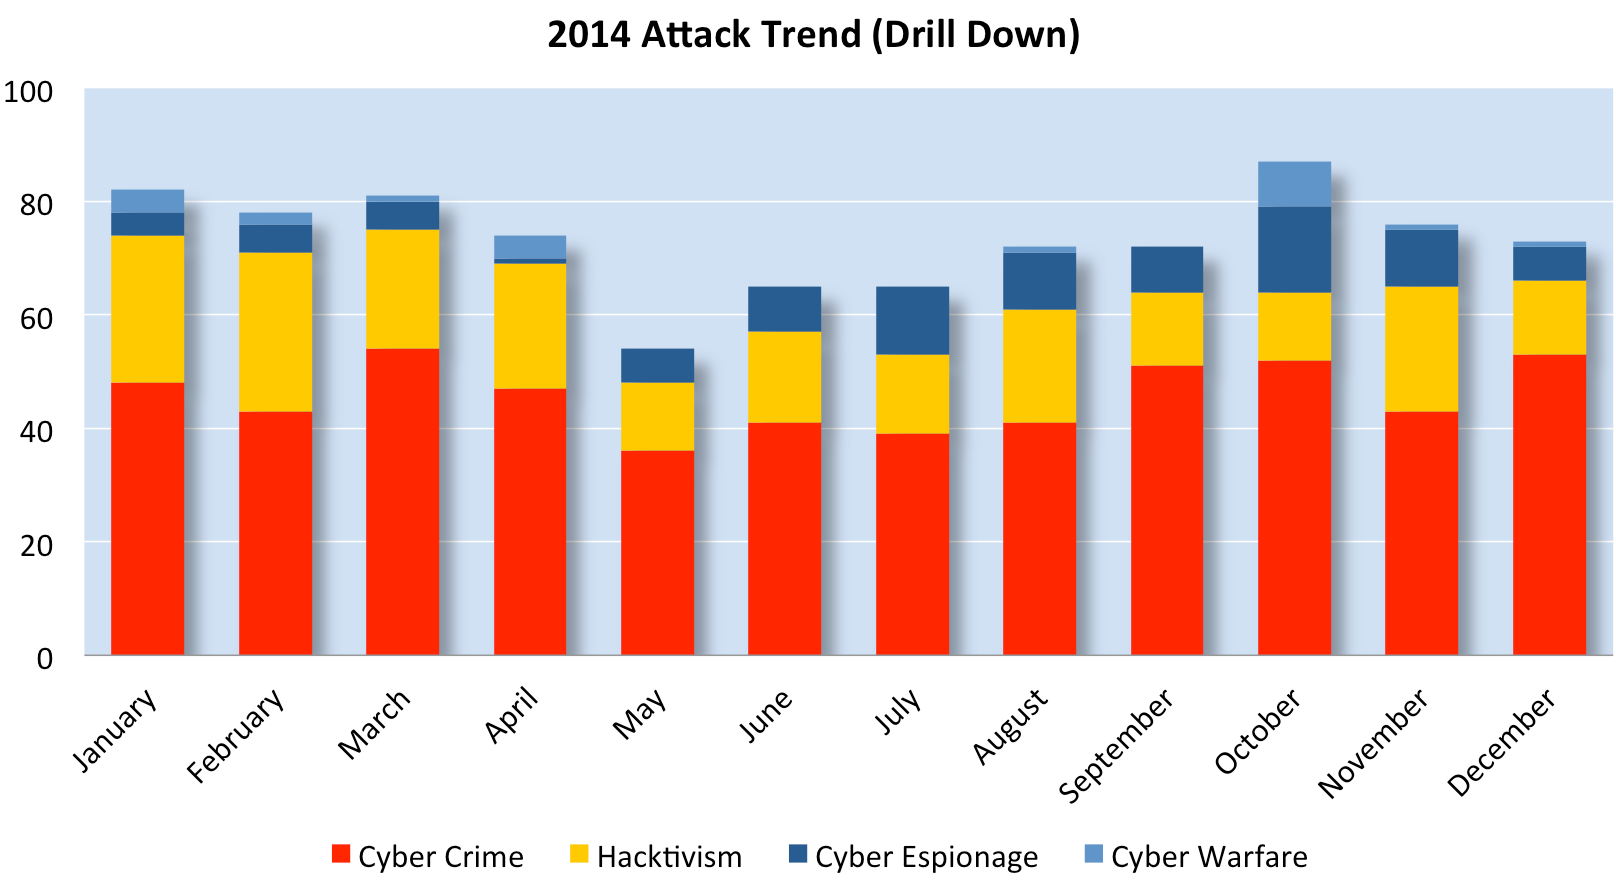
\includegraphics[scale=0.2]{Imagens/hackmageddon_trends.png}
		\caption{Difusão}
	\end{minipage}
	\begin{minipage}{.5\textwidth}
		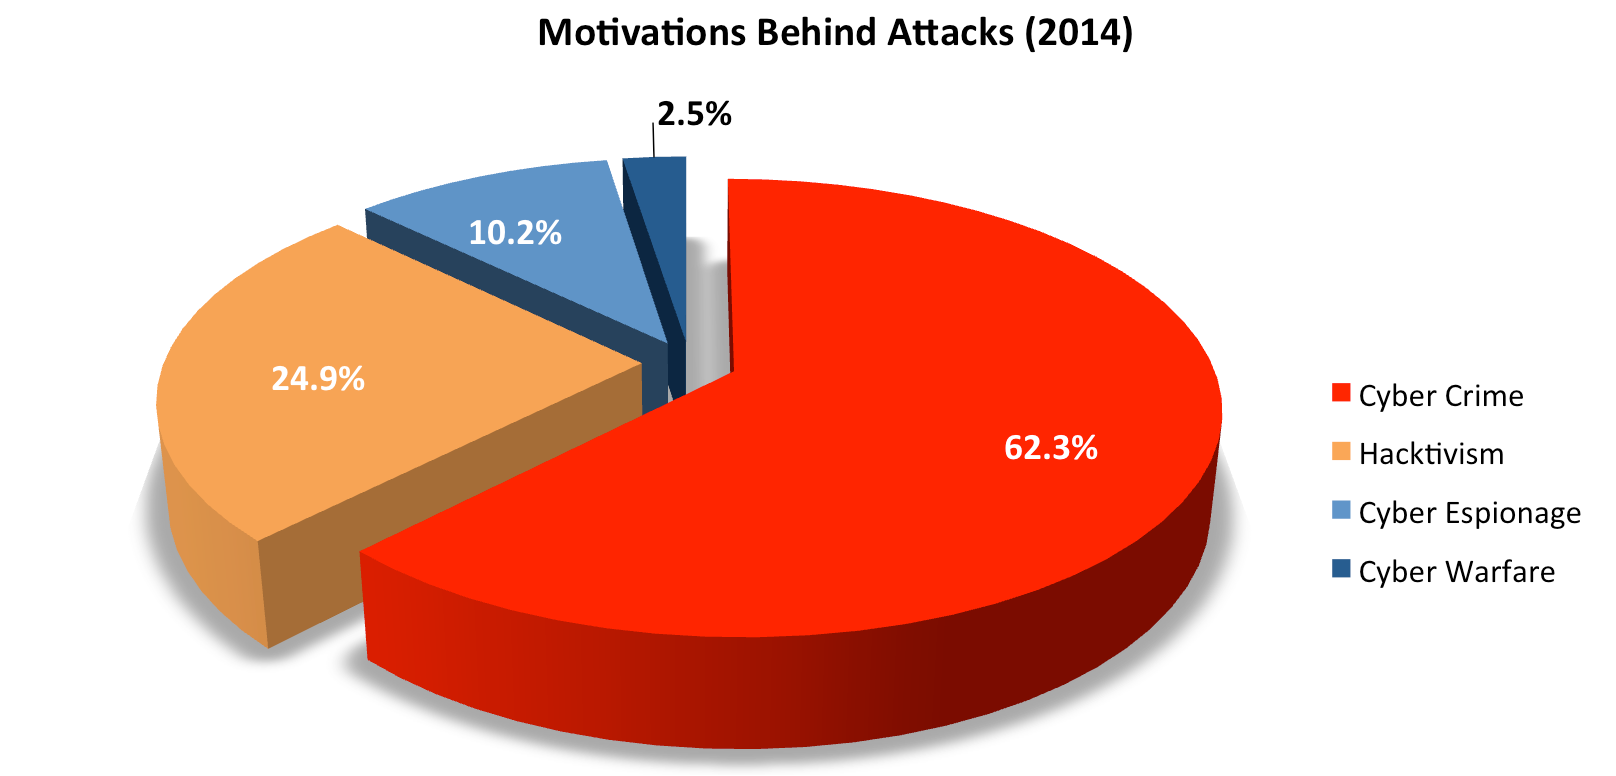
\includegraphics[scale=0.2]{Imagens/hackmageddon_motivation.png}
		\caption{Motivação}
	\end{minipage}
	\begin{minipage}{.5\textwidth}
		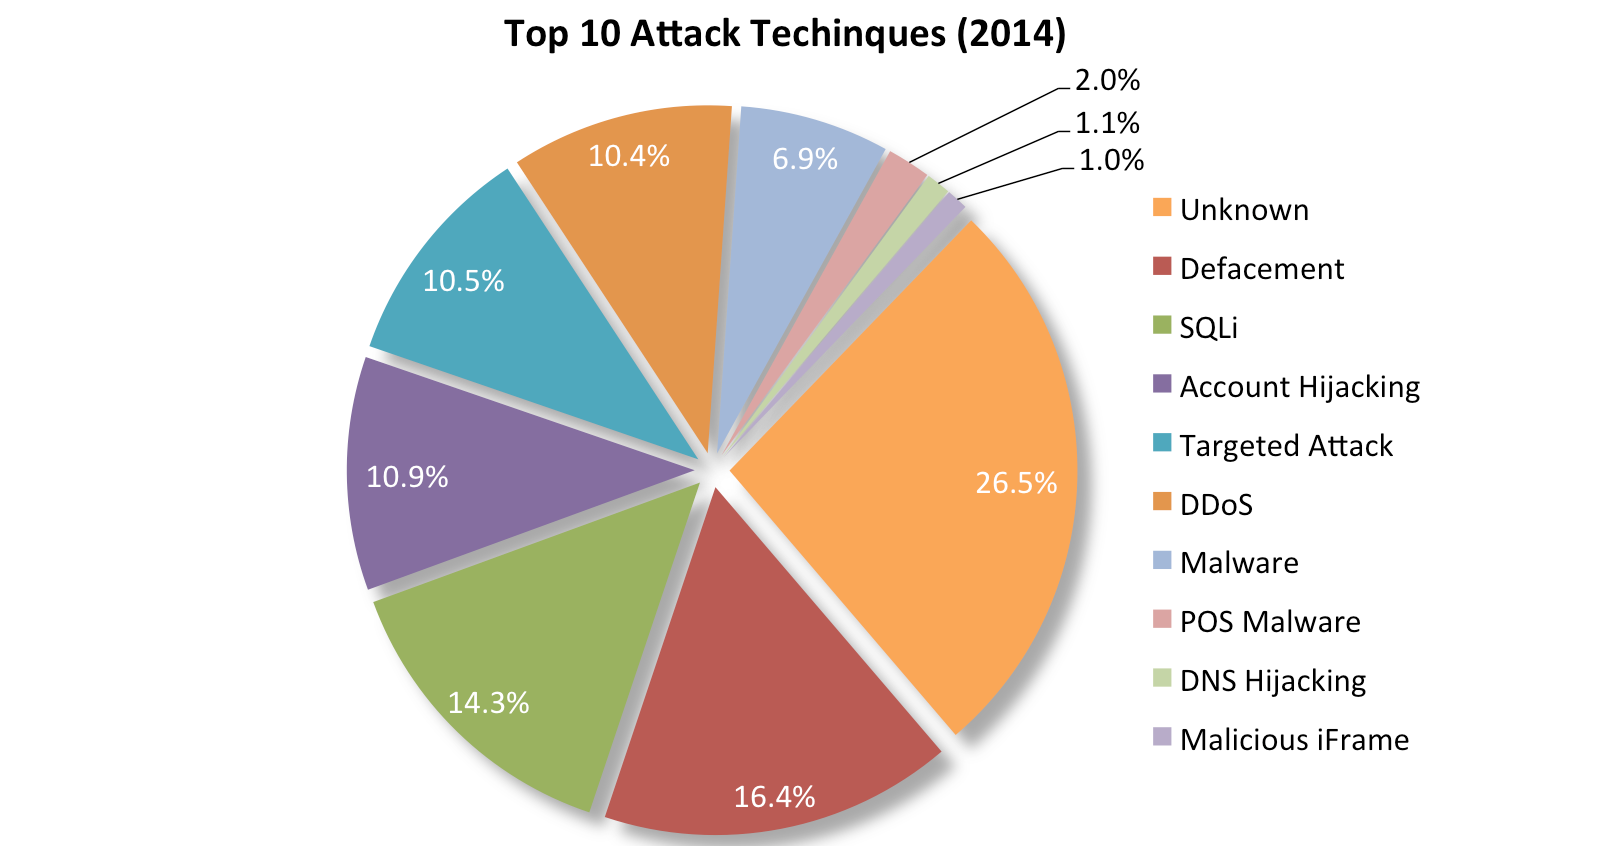
\includegraphics[scale=0.2]{Imagens/hackmageddon_techniques.png}
		\caption{Técnicas}
	\end{minipage}
	\begin{minipage}{.5\textwidth}
		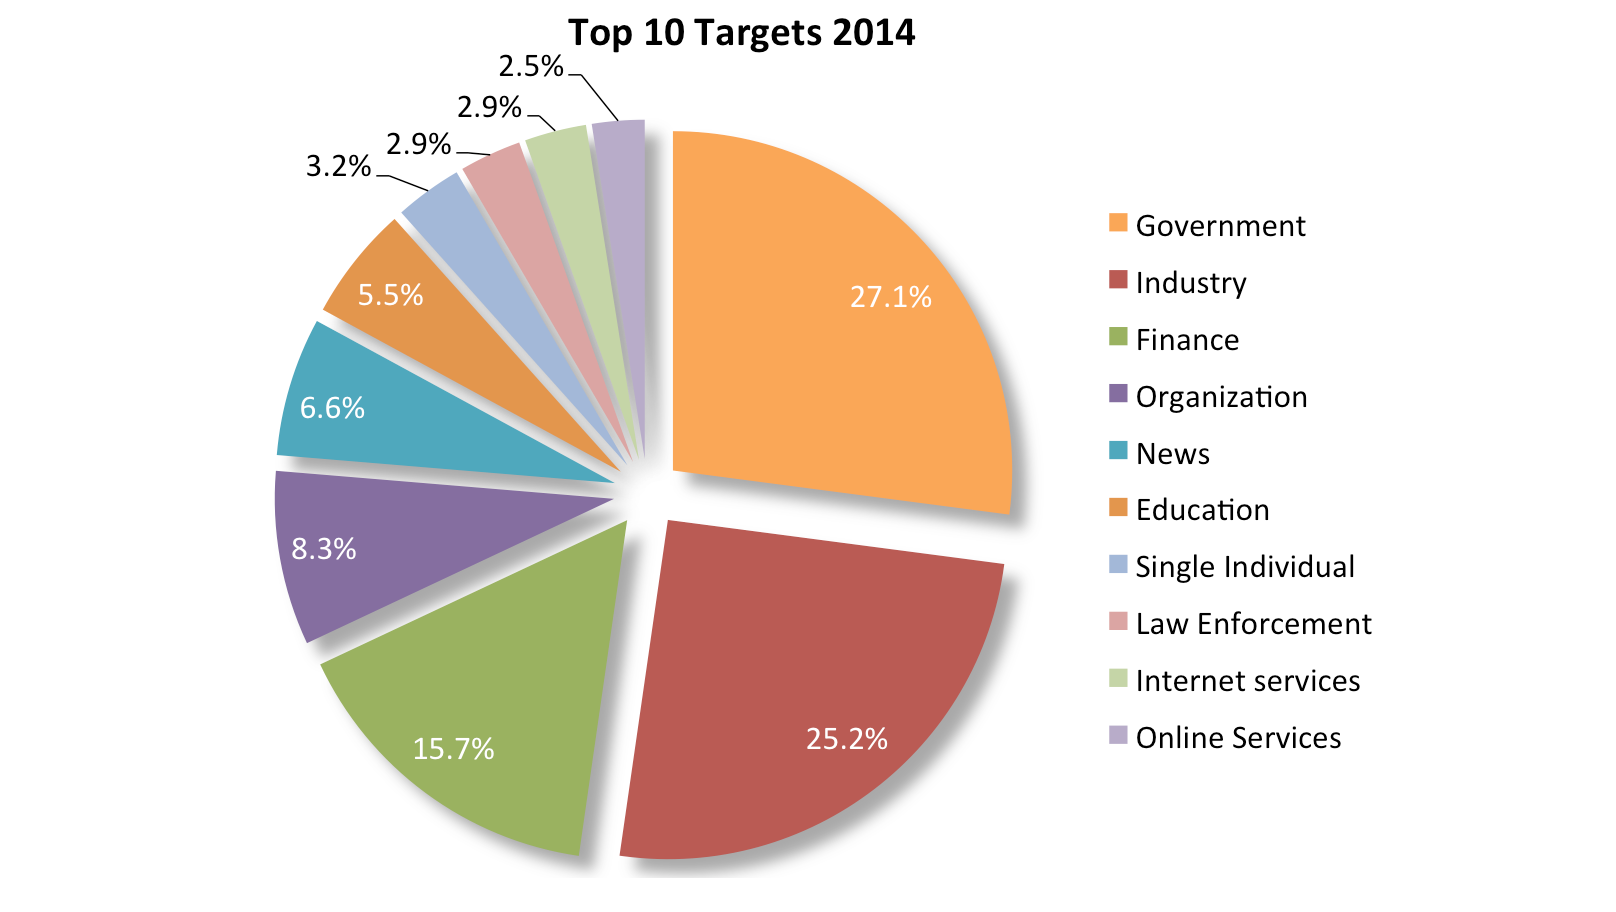
\includegraphics[scale=0.2]{Imagens/hackmageddon_targets.png}
		\caption{Alvos}
	\end{minipage}
\end{figure}

\begin{description} 
	\item[Figura 1] . 
	\item[Figura 2] .
	\item[Figura 3] .
	\item[Figura 4] The third etc 
	\ldots 
\end{description}

Os riscos são avaliados de acordo com as chances de um quebra de segurança  ocorrer e com os custos envolvidos para tratá-lo. Técnicas de defesa vêm sendo aprimoradas, porém ainda existem diversas limitações que as impedem de estarem efetivamente preparadas para o qualquer tipo de ataque \cite{CeC}, sendo assim necessário  soluções inovadoras para tratar os níveis de ameaças atuais e futuras. 

A necessidade de se proteger contra estes riscos de ataques acabou despertando interesse por ferramentas automatizadas para se detectá-los e preveni-los.

Este cenário é a principal motivação deste trabalho que consiste em propor, implementar e mensurar resultados de uma solução para treinamento de RNA para detecção e prevenção de intrusão.





\section{Escopo}

As ferramentas de detecção de intrusão são chamadas de IDS (Intrusion Detection System), seu trabalho é monitorar as atividades e analisar os eventos em uma rede em busca de anomalias que sugiram uma invasão. Estes não costumam executar qualquer ação para impedir intrusões, sua principal função é alertar os administradores de sistemas que há uma possível violação de segurança, sendo desta forma uma ferramenta passiva.
Existem as ferramentas de prevenção de intrusão, que são conhecidas como IPS (Intrusion Prevention System) estas são ferramentas que assim como IDS analisam o trafego e os eventos de uma rede, porem reagem de forma a bloquear o acesso ou atividade maliciosa, senso assim uma ferramenta ativa.

Podemos classificar os IDS da seguinte forma.

Baseado em Host ou rede, onde o primeiro faz uso de arquivos de log para cada computador individualmente e o segundo captura pacotes que trafegam na rede para analisar seu conteúdo.

Online ou Offline, onde um é capaz de detectar e marcar um intruso enquanto a esta sendo realizada a intrusão, e o outro analisa registros após o evento ocorrer e indica que houve uma violação de segurança tinha ocorrido desde a última verificação, respectivamente.

Baseado em abuso ou anomalia, onde por anomalia o sistema identifica comportamento fora do padrão, e por abuso compara as atividades na rede com comportamentos de ataques já conhecidos.

A maioria dos métodos utilizados para detecção são baseados em inteligencia artificial (AI), entre as varias técnicas conhecidas de AI, a que tem tido melhores resultados e consequentemente mais usada é a de Redes Neurais Artificiais (RNA)\cite{Jake-Ryan}\cite{Stampar}.

As RNA são uma classe de algorítimos para aprendizado de maquina (AM), usada para realizar classificação de dados. A rede neural é treinada de forma a dar mais importância para as principais características de uma determinada instancia de um problema, para ajudar a classificar os dados que ainda estão por vir. 
RNAs tem sido utilizadas com sucesso na detecção de intrusão \cite{Zhang} \cite{Tong} \cite{Wonil}, porem elas necessitam de uma quantidade substancial de dados para realizar o treinamento, a partir desse treinamento que ela passara a ter capacidade de identificar os padrões para posteriormente receber os dados novos para classificação.




\section{Justificativa}

Muitas técnicas de AI tem sido utilizadas para IDS/IPS, a mais utilizada e a RNA\cite{Stampar}, porem existem tipos de ataques que não são facilmente detectados, por ocorrerem com menor frequência, tendo poucas entradas para o treino da RNA\cite{CeC}, resultando em mais erros,  por esse motivo escolhemos trabalhar de forma a aprimorar seus resultados. 


\section{Objetivos}

O objetivo deste trabalho é propor uma forma de aprimorar o sistema de aprendizado de redes neurais artificiais para detecção e prevenção de intrusão. 
Para isso sera necessário, gerar uma base em um ambiente controlado para testes específicos, implementar uma solução de IPS/IDS que utilize RNA, implementar uma metodologia de treinamento, realizar o treino da RNA e por fim comparar resultados com outras técnicas de treinamento para RNA.


\section{Método de trabalho}

Utilizaremos a base de dados de trafego em rede KDD Cup 99\cite{KDDCup99}, por ser uma das bases mais completas e amplamente utilizada nos testes de IDS, sera essencial para se realizar uma comparação consistente de resultados.

Para gerar nossa base mais especifica iremos monitorar um ambiente de rede durante um período de tempo, no qual serão realizados alguns ataques controlados periodicamente, deste sera gerado um log que usaremos no nosso sistema.

Desenvolver uma solução para analise dos pacotes e eventos de uma rede, esta sera desenvolvida em Go, utilizara RNA para classificar as atividades na rede.

Realizar treinamento em ambas as bases de dados, serão formas diversificadas de treinamento, sera feito uma comparação de acertos/erros e tempo necessário para treino.

Faremos uma comparação de desempenho e efetividade de nossa solução e algumas que temos hoje.

\section{Organização do trabalho}

Este trabalho esta dividido em trés partes.
Na próxima seção, sera apresentado o estado da arte, onde sera revisado a literatura sobre detecção e prevenção de intrusão utilizando RNA.

Logo apos teremos a proposta  de forma mais detalhada do que é pretendido realizar na próxima etapa do trabalho.

Por fim um cronograma de controle sobre como prosseguira a segunda etapa deste trabalho.



% ----------------------------------------------------------
% Capitulo 2
% ----------------------------------------------------------
\chapter[Revisão de Literatura]{Revisão de Literatura}
%\addcontentsline{toc}{chapter}{Revisão de Literatura}
% ----------------------------------------------------------

No trabalho de Roberto Silva \cite{RobertoSilva} explica que IDS é um um software com a função de identificar, detectar e responder a atividades anormais e nao autorizadas em um sistema. Para entender melhor o que é “Detecção de intrusão”, é preciso entender o que é uma intrusão. A palavra intrusão é definida no dicionário como “o ato de empurrar, ou entrar em um lugar ou estado sem ser convidado, sem ter direito ou ser bem vindo.”. Na computação é simplesmente uma atividade não autorizada no sistema ou na rede por um de seus computadores ou redes de computadores. O funcionamento de um IDS depende do local em que ele é colocado na rede, sendo classificado de 3 formas. Sistema de Detecção de Intrusão Baseado em Rede (NIDS)...

No trabalho de Marley  \cite{Marley}, é dada uma visão geral sobre Redes Neurais Artificiais(RNA), explicando que a expressão "rede neural" é a tentativa de representar a capacidade que cérebro humano possui de reconhecer, associar e generalizar padrões, sendo as principais áreas de atuação para a classificação de padrões e previsão.A modelagem de uma rede neural consiste em três etapas: (1) Treinamento e Aprendizado, obtido pelo ambiente gerador dos dados, (2) Associação, obtido pelo reconhecimento de padrões distintos e (3) Generalização, relacionado a capacidade da rede de reconhecer com sucesso o ambiente que origina os dados, não propriamente os dados utilizados no treinamento.O conhecimento é passado por um algoritmo de treinamento e aprendizado, este é transformado e armazenado nas conexões. O aprendizado é resultado de muitas apresentações de conjuntos de exemplos de treinamento.O treinamento pode ser dado de duas maneiras: (1)batelada ou ciclos, onde a atualização somente acontece depois da apresentação de todos os pesos e (2) padrão a padrão ou incremental,onde a atualização é feita após a apresentação de cada novo padrão. O procedimento de treinamento pode ser classificado em dois tipos: supervisionado e não supervisionado.

Para mostrar a importância de técnicas de inteligência artificial para detecção de intrusão no trabalho feito na Information Systems Security Bureau \cite{InformationSustem}, foi feito uma analise quantitativa na forma de pesquisa cientifica dando uma visão geral da literatura procurando publicações com tópicos relacionados a “Detecção de intrusão”. 
Com o objetivo principal da pesquisa sendo uma forma compreensível de mostrar as tendências atuais na área. 
Foi utilizado o Google Acadêmico por ser aberto e simples, para realizar as pesquisas na literatura cientifica. 
A primeira comparação é  do período de 2010 a 2014, utilizando um auxiliar “Outros” que seria, por exemplo, detectores de intrusão baseados em assinaturas, e comparando com os baseados em aprendizado de maquina e inteligência artificial, mesmo Outros tendo muito mais publicações, é possível ver um aumento significativo nas duas técnicas nos últimos anos.
A segunda comparação também no período de 2010 a 2014, mostrando diferentes algoritmos de inteligência artificial utilizados para detecção de intrusão, entre eles estão: Redes Neurais, Lógica Fuzzy, Algoritmos Genéticos, Arvores de Decisão, Support Vector Machies e entre outros. 
Redes neurais, com um grande vantagem sobre os outros algoritmos, se mostrando o algoritmo de inteligência artificial mais popular na literatura ciência, mas a resultados promissores em técnicas híbridas, onde se utiliza diferentes técnicas de inteligência artificiais combinadas.

No trabalho em conjunto do Departamento de Automação e Sistemas da Universidade Federal de Santa Catarina \cite{polvo1} e com a Pontifícia Universidade Católica do Paraná \cite{polvo2}, foi desenvolvido um modelo multi-camadas chamado de POLVO-IIDS, sendo uma técnica híbrida que combina redes neurais com Support Vector Machies(SVM). Com o objetivo principal de prover um sistema de detecto de intrusão inteligente (IIDS) que seja preciso, flexível, tolerante a variações de ataques, adaptativo a variações de ambiente, modular e que atue em tempo real.
O modelo consiste em duas camadas: 
A primeira camada é o classificador, composta de uma rede neural de Kohonen, fazendo uma pre-seleção do trafego de entrada, através da analise de características contidas nos pacotes em um determinado período de tempo e indicando como saída se é uma intrusão ou normal.
A segunda camada é detector de anomalias, composto por quatro Support Vector Machines, cada um trata de uma categoria distinta de ataque, sendo especializado no tipo correspondente e com duas opções de saída: trafego normal ou atividade maliciosa. As categorias usadas na criação do detector de anomalias foram: DoS, Worm, Scan, R2L/Normal.
O protótipo foi implementado utilizando a linguagem de programação Java e a rede neural de Kohonen e as SVMs foram implementadas no framework Joone (Java Object Oriented Neural Engine Versão 2.0).
Os resultados obtidos com os testes, mostrou que o modelo é eficiente, usando a base de dados KDD Cup 1999 Data,foram efetuados quatro testes para medir as taxas de acerto. Os testes 1 e 2 contaram com 15000 e 30000 dados de entrada, respectivamente, para treinamento da rede com reforço de 100 vezes para cada entrada. Os testes 3 e 4 utilizando os mesmos dados de entrada, porem com reforço de 1000 vezes para cada entrada. O teste 4 se mostrou o mais eficiente utilizando 30000 entradas e reforço de 1000 vezes para cada entrada, teve uma taxa de acerto médio de 96,55\%, embora tenha levado cerca de 40 minutos.


Muitas abordagens de RNA tem sido implementadas e testadas para IDS, um sistema proposto por Ryan \cite{Ryan}, analisou  o comportamento de usuários individuais. O padrão de entrada foi então combinado com os perfis de usuário para identificar o utilizador (Um nó correspondente ao utilizador com um valor > 0,5 é atribuída a esse usuário). Um flag é gerado se nenhuma correspondência for encontrada,  este é considerado como uma anomalia. No entanto, isto exigia grande quantidade de dados para treinar a rede para cada utilizador. Dados insuficientes para um usuário pode levar à falsos positivos para o comportamento desse usuário na rede. O sistema teve uma taxa de detecção de anomalia de 96\% e 7\% de falsos alarmes.

Cannady propôs um modelo chamado Multi-layered Perceptron (MLP) \cite{Cannady}, utilizando o algorítimo de \textit{backpropagation} ao invés de criar perfis individuais. Foi necessário 26.13 horas para completar com aproximadamente 98\% de acerto no conjunto de dados de treinamento e 97,5\% no conjunto de dados de teste.

Devaraju e Ramakrishnan implementaram a  Rede Neural Probabilística (PNN) \cite{Devaraju} esta obteve desempenho melhor do que uma rede do tipo FeedForward e Radial Basis. No entanto, a PNN (precisão = 80,38\%) conseguiu ser apenas 0,02\% melhor do que a rede do tipo FeedForward (precisão = 80,4\%) nao sendo uma diferença significativa. A precisão do  Radial Basis é de 75,4\%.
Resultados mais baixos que as abordagens que vimos até agora.

Shraddha Surana propôs um modelo \cite{Surana} utilizando clusterização Fuzzy e Redes neurais artificiais, onde o dataset de treinamento é dividido em N subsets, que são distribuídos em N redes neurais intermediarias, com mais uma camada de RNA que agrega os resultados das redes intermediarias para a partir dai realizar a classificação de novos dados. Esta abordagem conseguiu uma taxa de detecção de 81,6\%.

Um trabalho feito na Pontifícia Universidade Católica do Rio de Janeiro \cite{RenatoMaia}, demonstra um teste de desempenho para algumas diferentes entradas para o treinamento de Redes neurais artificiais.

Utilizando 4 redes e no máximo 4 saídas possíveis, é testado diferentes composições, de forma a encontrar uma ideal maneira de treinamento de uma rede neural, utilizando as 41 categorias disponíveis.
As 4 são categorizas como Normal ou entre 3 tipos de ataque DoS Smurf, Nepture ou Back.
A primeira rede utiliza 9 entradas e uma saídas, onde a saída pode ser -1 para normal e 1 para ataque.
A segunda rede utiliza todas as 41 entradas e uma saída, onde a saída pode ser -1 para normal e 1 para ataque.
A terceira utiliza nove entradas e uma saída, onde a saída pode ser -1 para normal,0 para Neptune e 1 Smurf.
A quarta e ultima rede, usa 9 entradas e quatro saídas que são organizadas em (-1 1 1 1) para Normal,(1 -1 1 1) para Neptune,(1 1 -1 1) para Back e (1 1 1 -1) para Smurf.

Utilizando a base de dados KDD Cup 1999 para o treinamento das redes neurais, os resultados foram bons e com baixa taxa de falsos positivos, as taxas de acertos foram acima de 90\% para todas as configurações testadas, a rede que teve um melhor resultado foi a terceira rede, tendo 97,5\% na sua taxa de acertos contra.

No trabalho feito na universidade de Waterloo no canada\cite{Chunlin}, foi apresentado duas técnicas de redes neurais baseados em hierarquia para IDS, hierarquia em series e hierarquia paralela, onde o objeto para a detecção de ataques de abuso e anomalia em tempo real sem a interrupção humana.

Usando dois pré-requisitos para redes neurais hierarquias. O primeiro, cada classificação individual deve acertar seu desempenho, caso contrario,o erro é enviado para os níveis acima, acumulando e influenciados os níveis mais baixos. A taxa de detecção e de falso positivo são os principais indicadores de desempenho. 

A segunda, as classificações,basicamente, podem ser dividas em grupos seguindo alguns critérios, cada grupo pode ser associado para seu própria classificação, então as classificações ou sua saída pode ser combinada em conjuntos.

O artigo conclui em seus resultados, uma ótima habilidade para detectar instruções conhecidas e desconhecidas com um curte período de tempo para o treinamento, uma alta taxa de detecção e um baixo índice de falsos positivos.
O IDS de hierarquia de series conseguiu monitorar em tempo real o trafego na rede, treinando automaticamente novas intrusos modificando sua estrutura para novas classificações. O IDS de hierarquia paralela, resolveu em partes, os problemas da hierarquia em series, sendo mais rápido para ser executado.



% ----------------------------------------------------------
% Capitulo 3
% ----------------------------------------------------------

\chapter[Proposta]{Proposta}
%\addcontentsline{toc}{chapter}{Metodologia}
% ----------------------------------------------------------

Será implementada na próxima etapa desse trabalho um modelo para Detecção e prevenção de intrusão fazendo uso de técnicas de inteligência artificial, especificamente redes neurais artificiais, utilizar suas características de reconhecimento de padrões e generalização para realizar a classificação dos eventos ocorridos em redes de computadores, classificando-os em normais ou intrusivos.

Será desenvolvida uma aplicação baseada no modelo, ela ira monitorar os pacotes em uma rede de computadores do tipo IPv4, este ira classificar e prevenir atividades maliciosas.

A principio será utilizada uma RNA do tipo \textit{feed-foward}, com três camadas apenas, uma de entrada, uma intermediaria e uma de saída. Os dados serão passados para a camada de entrada, processados pela rede e classificados como uma das cinco classes da camada de saída. Estas sendo Normal, DoS, U2R, R2L e Probe.  

O modelo terá foco no treinamento da RNA, a principio para aprender os pesos da rede em multicamadas sera usado o algorítimo de \textit{backpropagation} com a regra de atualização de peso do gradiente descendente.

Desse ponto serão mensurados alguns testes a partir da abordagem do POLVO-IIDS \cite{polvo1}, no qual usaremos uma rede para classificação, e quatro SVM para detecção de anomalias.

Outra abordagem é a de clusterização \cite{Surana}, separando o \textit{dataset} de treino em N \textit{subsets}, cada um sera utilizado para realizar o treinamento de uma rede neural, para no final outra rede  realizar a agregação dos resultados destas N redes.

 
Pretende-se analisar a viabilidade de aplicação destas abordagens, bem como
detalhar suas vantagens ou desvantagens em relação a métodos convencionais de
detecção de intrusão.


% ----------------------------------------------------------
% Capitulo 4
% ----------------------------------------------------------


\chapter[Cronograma]{Cronograma}
%\addcontentsline{toc}{chapter}{Expectativas}
% ---

Para modelar a proposta descrita, sera seguido um cronograma semanal, este ira descrever semana a semana as tarefas que devem ser realizadas de forma a se concluir o trabalho.


\vspace{.25cm}
\begin{center}
	\begin{tabular}{ |c| p{13.5cm} | }
		\hline
		\textbf{Semana} & \textbf{Atividade} \\ \hline \hline
		$1^{\underline a}$ & Analise de trafego de pacotes em rede, criar aplicação em Go para ler e realizar log das operações na rede \\ \hline
		$2^{\underline a}$ & Criar base de dados de trafego em rede de forma controlada. Verificar como implementações de IDS atuais reagem a esses dados. / trabalhar na monografia \\ \hline
		$3^{\underline a}$ & Implementar na aplicação de log de trafego um sistema de redes neurais \\ \hline		
		$4^{\underline a}$ & Realizar treinamento da RNA da aplicação com os \textit{datasets} KDD'99 e o modelado para o projeto / trabalhar na monografia \\ \hline		
		$5^{\underline a}$ & Mensurar resultados da aplicação do modelo / trabalhar na monografia \\ \hline		
		$6^{\underline a}$ & Comparar com os resultados obtidos por outros IDS, e com resultados publicados de outros modelos baseados em RNA  \\ \hline		
		$7^{\underline a}$ & Analisar se for possível como aprimorar os resultados do modelo \\ \hline		
		$8^{\underline a}$ & Implementar o modelo de POLVO-IIDS \\ \hline		
		$9^{\underline a}$ & Comparar com os resultados obtidos anteriormente / trabalhar na monografia \\ \hline		
		$10^{\underline a}$ & Implementar RNA clusterizado. \\ \hline		
		$11^{\underline a}$ & Comparar com os resultados obtidos anteriormente / trabalhar na monografia \\ \hline		
		$13^{\underline a}$ & Implementar modelo hibrido POLVO-IIDS Clusterizado \\ \hline		
		$14^{\underline a}$ & Comparar com os resultados obtidos anteriormente / trabalhar na monografia \\ \hline		
		$15^{\underline a}$ & Trabalhar na monografia - desenvolvimento \\ \hline		
		$16^{\underline a}$ & Trabalhar na monografia - resultados \\ \hline		
		$17^{\underline a}$ & Trabalhar na monografia - resultados \\ \hline		
		$18^{\underline a}$ & Apresentação dos resultados \\ \hline
		\end{tabular}
\end{center}

\vspace{1.25cm}


% ----------------------------------------------------------
% ELEMENTOS PÓS-TEXTUAIS
% ----------------------------------------------------------
\postextual
% ----------------------------------------------------------

% ----------------------------------------------------------
% Referências bibliográficas
% ----------------------------------------------------------
\bibliography{mono}


% Revisao Bibliografica
\end{document}
